% Generated by Sphinx.
\def\sphinxdocclass{report}
\documentclass[letterpaper,10pt,english]{sphinxmanual}
\usepackage[utf8]{inputenc}
\DeclareUnicodeCharacter{00A0}{\nobreakspace}
\usepackage{cmap}
\usepackage[T1]{fontenc}
\usepackage{babel}
\usepackage{times}
\usepackage[Bjarne]{fncychap}
\usepackage{longtable}
\usepackage{sphinx}
\usepackage{multirow}


\title{eurobot Documentation}
\date{December 05, 2014}
\release{}
\author{Author}
\newcommand{\sphinxlogo}{}
\renewcommand{\releasename}{Release}
\makeindex

\makeatletter
\def\PYG@reset{\let\PYG@it=\relax \let\PYG@bf=\relax%
    \let\PYG@ul=\relax \let\PYG@tc=\relax%
    \let\PYG@bc=\relax \let\PYG@ff=\relax}
\def\PYG@tok#1{\csname PYG@tok@#1\endcsname}
\def\PYG@toks#1+{\ifx\relax#1\empty\else%
    \PYG@tok{#1}\expandafter\PYG@toks\fi}
\def\PYG@do#1{\PYG@bc{\PYG@tc{\PYG@ul{%
    \PYG@it{\PYG@bf{\PYG@ff{#1}}}}}}}
\def\PYG#1#2{\PYG@reset\PYG@toks#1+\relax+\PYG@do{#2}}

\expandafter\def\csname PYG@tok@vg\endcsname{\def\PYG@tc##1{\textcolor[rgb]{0.73,0.38,0.84}{##1}}}
\expandafter\def\csname PYG@tok@bp\endcsname{\def\PYG@tc##1{\textcolor[rgb]{0.00,0.44,0.13}{##1}}}
\expandafter\def\csname PYG@tok@gp\endcsname{\let\PYG@bf=\textbf\def\PYG@tc##1{\textcolor[rgb]{0.78,0.36,0.04}{##1}}}
\expandafter\def\csname PYG@tok@si\endcsname{\let\PYG@it=\textit\def\PYG@tc##1{\textcolor[rgb]{0.44,0.63,0.82}{##1}}}
\expandafter\def\csname PYG@tok@sx\endcsname{\def\PYG@tc##1{\textcolor[rgb]{0.78,0.36,0.04}{##1}}}
\expandafter\def\csname PYG@tok@kn\endcsname{\let\PYG@bf=\textbf\def\PYG@tc##1{\textcolor[rgb]{0.00,0.44,0.13}{##1}}}
\expandafter\def\csname PYG@tok@kp\endcsname{\def\PYG@tc##1{\textcolor[rgb]{0.00,0.44,0.13}{##1}}}
\expandafter\def\csname PYG@tok@sc\endcsname{\def\PYG@tc##1{\textcolor[rgb]{0.25,0.44,0.63}{##1}}}
\expandafter\def\csname PYG@tok@ni\endcsname{\let\PYG@bf=\textbf\def\PYG@tc##1{\textcolor[rgb]{0.84,0.33,0.22}{##1}}}
\expandafter\def\csname PYG@tok@c\endcsname{\let\PYG@it=\textit\def\PYG@tc##1{\textcolor[rgb]{0.25,0.50,0.56}{##1}}}
\expandafter\def\csname PYG@tok@no\endcsname{\def\PYG@tc##1{\textcolor[rgb]{0.38,0.68,0.84}{##1}}}
\expandafter\def\csname PYG@tok@ne\endcsname{\def\PYG@tc##1{\textcolor[rgb]{0.00,0.44,0.13}{##1}}}
\expandafter\def\csname PYG@tok@sb\endcsname{\def\PYG@tc##1{\textcolor[rgb]{0.25,0.44,0.63}{##1}}}
\expandafter\def\csname PYG@tok@sr\endcsname{\def\PYG@tc##1{\textcolor[rgb]{0.14,0.33,0.53}{##1}}}
\expandafter\def\csname PYG@tok@sd\endcsname{\let\PYG@it=\textit\def\PYG@tc##1{\textcolor[rgb]{0.25,0.44,0.63}{##1}}}
\expandafter\def\csname PYG@tok@mo\endcsname{\def\PYG@tc##1{\textcolor[rgb]{0.13,0.50,0.31}{##1}}}
\expandafter\def\csname PYG@tok@nv\endcsname{\def\PYG@tc##1{\textcolor[rgb]{0.73,0.38,0.84}{##1}}}
\expandafter\def\csname PYG@tok@ge\endcsname{\let\PYG@it=\textit}
\expandafter\def\csname PYG@tok@gu\endcsname{\let\PYG@bf=\textbf\def\PYG@tc##1{\textcolor[rgb]{0.50,0.00,0.50}{##1}}}
\expandafter\def\csname PYG@tok@gr\endcsname{\def\PYG@tc##1{\textcolor[rgb]{1.00,0.00,0.00}{##1}}}
\expandafter\def\csname PYG@tok@nb\endcsname{\def\PYG@tc##1{\textcolor[rgb]{0.00,0.44,0.13}{##1}}}
\expandafter\def\csname PYG@tok@nd\endcsname{\let\PYG@bf=\textbf\def\PYG@tc##1{\textcolor[rgb]{0.33,0.33,0.33}{##1}}}
\expandafter\def\csname PYG@tok@m\endcsname{\def\PYG@tc##1{\textcolor[rgb]{0.13,0.50,0.31}{##1}}}
\expandafter\def\csname PYG@tok@kr\endcsname{\let\PYG@bf=\textbf\def\PYG@tc##1{\textcolor[rgb]{0.00,0.44,0.13}{##1}}}
\expandafter\def\csname PYG@tok@s\endcsname{\def\PYG@tc##1{\textcolor[rgb]{0.25,0.44,0.63}{##1}}}
\expandafter\def\csname PYG@tok@w\endcsname{\def\PYG@tc##1{\textcolor[rgb]{0.73,0.73,0.73}{##1}}}
\expandafter\def\csname PYG@tok@gs\endcsname{\let\PYG@bf=\textbf}
\expandafter\def\csname PYG@tok@gi\endcsname{\def\PYG@tc##1{\textcolor[rgb]{0.00,0.63,0.00}{##1}}}
\expandafter\def\csname PYG@tok@kt\endcsname{\def\PYG@tc##1{\textcolor[rgb]{0.56,0.13,0.00}{##1}}}
\expandafter\def\csname PYG@tok@gh\endcsname{\let\PYG@bf=\textbf\def\PYG@tc##1{\textcolor[rgb]{0.00,0.00,0.50}{##1}}}
\expandafter\def\csname PYG@tok@cp\endcsname{\def\PYG@tc##1{\textcolor[rgb]{0.00,0.44,0.13}{##1}}}
\expandafter\def\csname PYG@tok@k\endcsname{\let\PYG@bf=\textbf\def\PYG@tc##1{\textcolor[rgb]{0.00,0.44,0.13}{##1}}}
\expandafter\def\csname PYG@tok@cs\endcsname{\def\PYG@tc##1{\textcolor[rgb]{0.25,0.50,0.56}{##1}}\def\PYG@bc##1{\setlength{\fboxsep}{0pt}\colorbox[rgb]{1.00,0.94,0.94}{\strut ##1}}}
\expandafter\def\csname PYG@tok@nl\endcsname{\let\PYG@bf=\textbf\def\PYG@tc##1{\textcolor[rgb]{0.00,0.13,0.44}{##1}}}
\expandafter\def\csname PYG@tok@o\endcsname{\def\PYG@tc##1{\textcolor[rgb]{0.40,0.40,0.40}{##1}}}
\expandafter\def\csname PYG@tok@mf\endcsname{\def\PYG@tc##1{\textcolor[rgb]{0.13,0.50,0.31}{##1}}}
\expandafter\def\csname PYG@tok@gt\endcsname{\def\PYG@tc##1{\textcolor[rgb]{0.00,0.27,0.87}{##1}}}
\expandafter\def\csname PYG@tok@il\endcsname{\def\PYG@tc##1{\textcolor[rgb]{0.13,0.50,0.31}{##1}}}
\expandafter\def\csname PYG@tok@kc\endcsname{\let\PYG@bf=\textbf\def\PYG@tc##1{\textcolor[rgb]{0.00,0.44,0.13}{##1}}}
\expandafter\def\csname PYG@tok@na\endcsname{\def\PYG@tc##1{\textcolor[rgb]{0.25,0.44,0.63}{##1}}}
\expandafter\def\csname PYG@tok@s1\endcsname{\def\PYG@tc##1{\textcolor[rgb]{0.25,0.44,0.63}{##1}}}
\expandafter\def\csname PYG@tok@nn\endcsname{\let\PYG@bf=\textbf\def\PYG@tc##1{\textcolor[rgb]{0.05,0.52,0.71}{##1}}}
\expandafter\def\csname PYG@tok@cm\endcsname{\let\PYG@it=\textit\def\PYG@tc##1{\textcolor[rgb]{0.25,0.50,0.56}{##1}}}
\expandafter\def\csname PYG@tok@nf\endcsname{\def\PYG@tc##1{\textcolor[rgb]{0.02,0.16,0.49}{##1}}}
\expandafter\def\csname PYG@tok@nc\endcsname{\let\PYG@bf=\textbf\def\PYG@tc##1{\textcolor[rgb]{0.05,0.52,0.71}{##1}}}
\expandafter\def\csname PYG@tok@nt\endcsname{\let\PYG@bf=\textbf\def\PYG@tc##1{\textcolor[rgb]{0.02,0.16,0.45}{##1}}}
\expandafter\def\csname PYG@tok@kd\endcsname{\let\PYG@bf=\textbf\def\PYG@tc##1{\textcolor[rgb]{0.00,0.44,0.13}{##1}}}
\expandafter\def\csname PYG@tok@sh\endcsname{\def\PYG@tc##1{\textcolor[rgb]{0.25,0.44,0.63}{##1}}}
\expandafter\def\csname PYG@tok@c1\endcsname{\let\PYG@it=\textit\def\PYG@tc##1{\textcolor[rgb]{0.25,0.50,0.56}{##1}}}
\expandafter\def\csname PYG@tok@vc\endcsname{\def\PYG@tc##1{\textcolor[rgb]{0.73,0.38,0.84}{##1}}}
\expandafter\def\csname PYG@tok@gd\endcsname{\def\PYG@tc##1{\textcolor[rgb]{0.63,0.00,0.00}{##1}}}
\expandafter\def\csname PYG@tok@mh\endcsname{\def\PYG@tc##1{\textcolor[rgb]{0.13,0.50,0.31}{##1}}}
\expandafter\def\csname PYG@tok@err\endcsname{\def\PYG@bc##1{\setlength{\fboxsep}{0pt}\fcolorbox[rgb]{1.00,0.00,0.00}{1,1,1}{\strut ##1}}}
\expandafter\def\csname PYG@tok@ow\endcsname{\let\PYG@bf=\textbf\def\PYG@tc##1{\textcolor[rgb]{0.00,0.44,0.13}{##1}}}
\expandafter\def\csname PYG@tok@mi\endcsname{\def\PYG@tc##1{\textcolor[rgb]{0.13,0.50,0.31}{##1}}}
\expandafter\def\csname PYG@tok@ss\endcsname{\def\PYG@tc##1{\textcolor[rgb]{0.32,0.47,0.09}{##1}}}
\expandafter\def\csname PYG@tok@s2\endcsname{\def\PYG@tc##1{\textcolor[rgb]{0.25,0.44,0.63}{##1}}}
\expandafter\def\csname PYG@tok@vi\endcsname{\def\PYG@tc##1{\textcolor[rgb]{0.73,0.38,0.84}{##1}}}
\expandafter\def\csname PYG@tok@se\endcsname{\let\PYG@bf=\textbf\def\PYG@tc##1{\textcolor[rgb]{0.25,0.44,0.63}{##1}}}
\expandafter\def\csname PYG@tok@go\endcsname{\def\PYG@tc##1{\textcolor[rgb]{0.20,0.20,0.20}{##1}}}

\def\PYGZbs{\char`\\}
\def\PYGZus{\char`\_}
\def\PYGZob{\char`\{}
\def\PYGZcb{\char`\}}
\def\PYGZca{\char`\^}
\def\PYGZam{\char`\&}
\def\PYGZlt{\char`\<}
\def\PYGZgt{\char`\>}
\def\PYGZsh{\char`\#}
\def\PYGZpc{\char`\%}
\def\PYGZdl{\char`\$}
\def\PYGZhy{\char`\-}
\def\PYGZsq{\char`\'}
\def\PYGZdq{\char`\"}
\def\PYGZti{\char`\~}
% for compatibility with earlier versions
\def\PYGZat{@}
\def\PYGZlb{[}
\def\PYGZrb{]}
\makeatother

\renewcommand\PYGZsq{\textquotesingle}

\begin{document}

\maketitle
\tableofcontents
\phantomsection\label{index::doc}


Contents:


\chapter{gui package}
\label{gui:gui-package}\label{gui:welcome-to-eurobot-s-documentation}\label{gui::doc}

\section{Submodules}
\label{gui:submodules}

\section{gui.communication module}
\label{gui:gui-communication-module}\label{gui:module-gui.communication}\index{gui.communication (module)}\index{CanTableControl (class in gui.communication)}

\begin{fulllineitems}
\phantomsection\label{gui:gui.communication.CanTableControl}\pysigline{\strong{class }\code{gui.communication.}\bfcode{CanTableControl}}
Bases: \code{PyQt4.QtGui.QWidget}

Controls what will be be shown in the CAN table
\index{add\_data() (gui.communication.CanTableControl method)}

\begin{fulllineitems}
\phantomsection\label{gui:gui.communication.CanTableControl.add_data}\pysiglinewithargsret{\bfcode{add\_data}}{\emph{msg\_frame}}{}
Puts a new CAN frame in the table
\begin{quote}\begin{description}
\item[{Parameters}] \leavevmode
\textbf{msg\_frame} -- new CAN frame

\item[{Returns}] \leavevmode
None

\end{description}\end{quote}

\end{fulllineitems}

\index{change\_typ\_filter() (gui.communication.CanTableControl method)}

\begin{fulllineitems}
\phantomsection\label{gui:gui.communication.CanTableControl.change_typ_filter}\pysiglinewithargsret{\bfcode{change\_typ\_filter}}{}{}
Runs a new filter on the table if the filter rules changed

\end{fulllineitems}

\index{run\_button\_clicked() (gui.communication.CanTableControl method)}

\begin{fulllineitems}
\phantomsection\label{gui:gui.communication.CanTableControl.run_button_clicked}\pysiglinewithargsret{\bfcode{run\_button\_clicked}}{}{}
Hides all filter options if new messages are received.

This is necessary because if the table is filtered while new rows are added the computer will be overloaded.

\end{fulllineitems}


\end{fulllineitems}

\index{EditHost (class in gui.communication)}

\begin{fulllineitems}
\phantomsection\label{gui:gui.communication.EditHost}\pysigline{\strong{class }\code{gui.communication.}\bfcode{EditHost}}
Bases: \code{PyQt4.QtGui.QWidget}

This widget is used to configure the connection to the robot

\end{fulllineitems}

\index{SendCan (class in gui.communication)}

\begin{fulllineitems}
\phantomsection\label{gui:gui.communication.SendCan}\pysigline{\strong{class }\code{gui.communication.}\bfcode{SendCan}}
Bases: \code{PyQt4.QtGui.QWidget}

This widget allows to send CAN messages from the robot
\index{selection\_changed() (gui.communication.SendCan method)}

\begin{fulllineitems}
\phantomsection\label{gui:gui.communication.SendCan.selection_changed}\pysiglinewithargsret{\bfcode{selection\_changed}}{}{}
This method updates the text in the fields

\end{fulllineitems}


\end{fulllineitems}

\index{Table (class in gui.communication)}

\begin{fulllineitems}
\phantomsection\label{gui:gui.communication.Table}\pysiglinewithargsret{\strong{class }\code{gui.communication.}\bfcode{Table}}{\emph{header}}{}
Bases: \code{PyQt4.QtGui.QTableWidget}

Draws a table and allows to add new rows and filter them.
\begin{quote}\begin{description}
\item[{Parameters}] \leavevmode
\textbf{header} -- header displayed on the top of the table

\end{description}\end{quote}
\index{add\_row() (gui.communication.Table method)}

\begin{fulllineitems}
\phantomsection\label{gui:gui.communication.Table.add_row}\pysiglinewithargsret{\bfcode{add\_row}}{\emph{data}, \emph{color}, \emph{autoscroll}, \emph{visible}}{}
Adds a new row to the table.
\begin{quote}\begin{description}
\item[{Parameters}] \leavevmode\begin{itemize}
\item {} 
\textbf{data} -- data for the new row

\item {} 
\textbf{color} (\emph{can.MsgColors}) -- color of the new row

\item {} 
\textbf{autoscroll} (\emph{bool}) -- defines if the table should scroll to the end.

\item {} 
\textbf{visible} (\emph{bool}) -- defines if the new row is visible or hidden

\end{itemize}

\item[{Returns}] \leavevmode


\end{description}\end{quote}

\end{fulllineitems}

\index{filter\_types() (gui.communication.Table method)}

\begin{fulllineitems}
\phantomsection\label{gui:gui.communication.Table.filter_types}\pysiglinewithargsret{\bfcode{filter\_types}}{\emph{types}}{}
Applies a filter to the list and hides unwanted rows
\begin{quote}\begin{description}
\item[{Parameters}] \leavevmode
\textbf{types} (\emph{bool{[}{]}}) -- defines which types should be visible

\item[{Returns}] \leavevmode
None

\end{description}\end{quote}

\end{fulllineitems}


\end{fulllineitems}

\index{TcpConnection (class in gui.communication)}

\begin{fulllineitems}
\phantomsection\label{gui:gui.communication.TcpConnection}\pysiglinewithargsret{\strong{class }\code{gui.communication.}\bfcode{TcpConnection}}{\emph{host}, \emph{port}}{}
Bases: \code{PyQt4.QtCore.QThread}

This thread receives and sends tcp data
\index{run() (gui.communication.TcpConnection method)}

\begin{fulllineitems}
\phantomsection\label{gui:gui.communication.TcpConnection.run}\pysiglinewithargsret{\bfcode{run}}{}{}
This endless loop is waiting for new data

\end{fulllineitems}


\end{fulllineitems}



\section{gui.field module}
\label{gui:gui-field-module}\label{gui:module-gui.field}\index{gui.field (module)}\index{GameField (class in gui.field)}

\begin{fulllineitems}
\phantomsection\label{gui:gui.field.GameField}\pysigline{\strong{class }\code{gui.field.}\bfcode{GameField}}
Bases: \code{PyQt4.QtGui.QWidget}

This class draws the Position of the Robots on a map.
\index{\_draw\_robot() (gui.field.GameField method)}

\begin{fulllineitems}
\phantomsection\label{gui:gui.field.GameField._draw_robot}\pysiglinewithargsret{\bfcode{\_draw\_robot}}{\emph{painter}, \emph{robot}, \emph{scale}}{}~\begin{quote}\begin{description}
\item[{Parameters}] \leavevmode\begin{itemize}
\item {} 
\textbf{painter} (\emph{QtGui.QPainter}) -- painter of the map

\item {} 
\textbf{robot} (\emph{dict}) -- data of the robot

\item {} 
\textbf{scale} (\emph{int}) -- scale of the map

\end{itemize}

\item[{Returns}] \leavevmode
None

\end{description}\end{quote}

\end{fulllineitems}

\index{paintEvent() (gui.field.GameField method)}

\begin{fulllineitems}
\phantomsection\label{gui:gui.field.GameField.paintEvent}\pysiglinewithargsret{\bfcode{paintEvent}}{\emph{event}}{}
Overrides method: \code{QtGui.paintEvent()}

This method is called every time the map is repainted.
The map is repainted every time one of the following things happens:
\begin{itemize}
\item {} 
the gui is opened

\item {} 
the window is resized

\item {} 
a robot moved and {\hyperref[gui:gui.field.GameField.setpoint]{\code{setpoint()}}} is called

\end{itemize}

\end{fulllineitems}

\index{setpoint() (gui.field.GameField method)}

\begin{fulllineitems}
\phantomsection\label{gui:gui.field.GameField.setpoint}\pysiglinewithargsret{\bfcode{setpoint}}{\emph{msg\_frame}}{}
This method checks if a CAN message contains the position of a Robot and actualise the position on the map.
\begin{quote}\begin{description}
\item[{Parameters}] \leavevmode
\textbf{msg\_frame} (\emph{dict}) -- CAN message

\item[{Returns}] \leavevmode
None

\end{description}\end{quote}

\end{fulllineitems}


\end{fulllineitems}



\section{gui.gui module}
\label{gui:module-gui.gui}\label{gui:gui-gui-module}\index{gui.gui (module)}\index{CanWindow (class in gui.gui)}

\begin{fulllineitems}
\phantomsection\label{gui:gui.gui.CanWindow}\pysigline{\strong{class }\code{gui.gui.}\bfcode{CanWindow}}
Bases: \code{PyQt4.QtGui.QWidget}
\index{connect\_host() (gui.gui.CanWindow method)}

\begin{fulllineitems}
\phantomsection\label{gui:gui.gui.CanWindow.connect_host}\pysiglinewithargsret{\bfcode{connect\_host}}{}{}
\end{fulllineitems}

\index{init\_ui() (gui.gui.CanWindow method)}

\begin{fulllineitems}
\phantomsection\label{gui:gui.gui.CanWindow.init_ui}\pysiglinewithargsret{\bfcode{init\_ui}}{}{}
\end{fulllineitems}

\index{lost\_connection() (gui.gui.CanWindow method)}

\begin{fulllineitems}
\phantomsection\label{gui:gui.gui.CanWindow.lost_connection}\pysiglinewithargsret{\bfcode{lost\_connection}}{}{}
\end{fulllineitems}


\end{fulllineitems}

\index{CreateGroupBox (class in gui.gui)}

\begin{fulllineitems}
\phantomsection\label{gui:gui.gui.CreateGroupBox}\pysiglinewithargsret{\strong{class }\code{gui.gui.}\bfcode{CreateGroupBox}}{\emph{widget}, \emph{text}}{}
Bases: \code{PyQt4.QtGui.QGroupBox}

\end{fulllineitems}

\index{main() (in module gui.gui)}

\begin{fulllineitems}
\phantomsection\label{gui:gui.gui.main}\pysiglinewithargsret{\code{gui.gui.}\bfcode{main}}{\emph{args}}{}
\end{fulllineitems}



\section{Module contents}
\label{gui:module-contents}\label{gui:module-gui}\index{gui (module)}

\chapter{kern package}
\label{kern::doc}\label{kern:kern-package}

\section{Structure}
\label{kern:structure}\begin{figure}[htbp]
\centering
\capstart

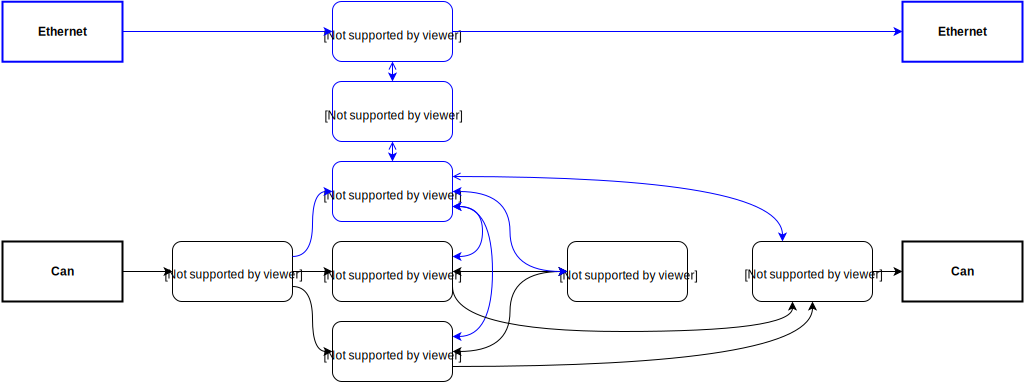
\includegraphics{kern_threads_1.svg}
\caption{Processes on Robot}\end{figure}


\section{Submodules}
\label{kern:submodules}

\section{kern.kern module}
\label{kern:module-kern.kern}\label{kern:kern-kern-module}\index{kern.kern (module)}\index{main() (in module kern.kern)}

\begin{fulllineitems}
\phantomsection\label{kern:kern.kern.main}\pysiglinewithargsret{\code{kern.kern.}\bfcode{main}}{}{}
Main programm running on Robot

\end{fulllineitems}



\section{Module contents}
\label{kern:module-kern}\label{kern:module-contents}\index{kern (module)}

\chapter{libraries package}
\label{libraries::doc}\label{libraries:libraries-package}
This module contains classes used to control hardware. It is used on the robot and on the computer.


\section{Submodules}
\label{libraries:submodules}

\section{libraries.can module}
\label{libraries:libraries-can-module}

\subsection{Example}
\label{libraries:example}\begin{quote}

Here a short example how to use the CAN interface:
First you have to create a new object:

\begin{Verbatim}[commandchars=\\\{\}]
\PYG{g+gp}{\PYGZgt{}\PYGZgt{}\PYGZgt{} }\PYG{n}{can\PYGZus{}connection} \PYG{o}{=} \PYG{n}{libraries}\PYG{o}{.}\PYG{n}{can}\PYG{o}{.}\PYG{n}{Can}\PYG{p}{(}\PYG{l+s}{\PYGZdq{}}\PYG{l+s}{can0}\PYG{l+s}{\PYGZdq{}}\PYG{p}{,} \PYG{n}{MsgSender}\PYG{o}{.}\PYG{n}{Debugging}\PYG{p}{)}
\end{Verbatim}

To send a message you have to put it in a dictionary:

\begin{Verbatim}[commandchars=\\\{\}]
\PYG{g+gp}{\PYGZgt{}\PYGZgt{}\PYGZgt{} }\PYG{n}{can\PYGZus{}msg} \PYG{o}{=} \PYG{p}{\PYGZob{}}
\PYG{g+go}{        \PYGZsq{}type\PYGZsq{}: can.MsgTypes.Position\PYGZus{}Robot\PYGZus{}1,}
\PYG{g+go}{        \PYGZsq{}position\PYGZus{}correct\PYGZsq{}: True,}
\PYG{g+go}{        \PYGZsq{}angle\PYGZus{}correct\PYGZsq{}: False,}
\PYG{g+go}{        \PYGZsq{}angle\PYGZsq{}: angle,}
\PYG{g+go}{        \PYGZsq{}y\PYGZus{}position\PYGZsq{}: y,}
\PYG{g+go}{        \PYGZsq{}x\PYGZus{}position\PYGZsq{}: x}
\PYG{g+go}{    \PYGZcb{}}
\PYG{g+gp}{\PYGZgt{}\PYGZgt{}\PYGZgt{} }\PYG{n}{can\PYGZus{}connection}\PYG{o}{.}\PYG{n}{send}\PYG{p}{(}\PYG{n}{can\PYGZus{}msg}\PYG{p}{)}
\end{Verbatim}

The received messages are taken from the buffer like this:

\begin{Verbatim}[commandchars=\\\{\}]
\PYG{g+gp}{\PYGZgt{}\PYGZgt{}\PYGZgt{} }\PYG{n}{can\PYGZus{}msg} \PYG{o}{=} \PYG{n}{can\PYGZus{}connection}\PYG{o}{.}\PYG{n}{queue\PYGZus{}position\PYGZus{}Robot\PYGZus{}1}\PYG{o}{.}\PYG{n}{get}\PYG{p}{(}\PYG{p}{)}
\end{Verbatim}
\end{quote}

\begin{notice}{note}{Note:}
There are 2 different ways to get the next value from a buffer:
\begin{itemize}
\item {} 
buffer.get()  This method waits for new data. The program is blocked.

\item {} 
buffer.get\_nowait()   This method returns None if there is no data available.

\end{itemize}
\end{notice}


\subsection{Description}
\label{libraries:module-libraries.can}\label{libraries:description}\index{libraries.can (module)}\index{Can (class in libraries.can)}

\begin{fulllineitems}
\phantomsection\label{libraries:libraries.can.Can}\pysiglinewithargsret{\strong{class }\code{libraries.can.}\bfcode{Can}}{\emph{interface}, \emph{sender}}{}
Bases: \code{builtins.object}

This Class allows to send and receive CAN messages

It starts 2 new threads. One for receiving and one for sending.
The incoming messages are decoded and put into multiple receive buffers.
Additionally all raw messages are put in the debug buffer.
\begin{quote}\begin{description}
\item[{Parameters}] \leavevmode\begin{itemize}
\item {} 
\textbf{interface} (\emph{str}) -- hardware Interface used to send

\item {} 
\textbf{sender} (\emph{MsgSender}) -- id of the Sender (defines the sender part in the CAN id)

\end{itemize}

\end{description}\end{quote}
\index{\_build\_can\_frame() (libraries.can.Can method)}

\begin{fulllineitems}
\phantomsection\label{libraries:libraries.can.Can._build_can_frame}\pysiglinewithargsret{\bfcode{\_build\_can\_frame}}{\emph{can\_id}, \emph{data}}{}
builds CAN frame
\begin{quote}\begin{description}
\item[{Parameters}] \leavevmode\begin{itemize}
\item {} 
\textbf{can\_id} -- 

\item {} 
\textbf{data} -- 

\end{itemize}

\item[{Returns}] \leavevmode
can\_frame

\end{description}\end{quote}

\end{fulllineitems}

\index{\_dissect\_can\_frame() (libraries.can.Can method)}

\begin{fulllineitems}
\phantomsection\label{libraries:libraries.can.Can._dissect_can_frame}\pysiglinewithargsret{\bfcode{\_dissect\_can\_frame}}{\emph{frame}}{}
reads CAN frame
\begin{quote}\begin{description}
\item[{Parameters}] \leavevmode
\textbf{frame} -- 

\item[{Returns}] \leavevmode
can\_id, can\_msg

\end{description}\end{quote}

\end{fulllineitems}

\index{\_recv\_connection() (libraries.can.Can method)}

\begin{fulllineitems}
\phantomsection\label{libraries:libraries.can.Can._recv_connection}\pysiglinewithargsret{\bfcode{\_recv\_connection}}{}{}
Never ending loop for receiving CAN messages

\end{fulllineitems}

\index{\_send\_connection() (libraries.can.Can method)}

\begin{fulllineitems}
\phantomsection\label{libraries:libraries.can.Can._send_connection}\pysiglinewithargsret{\bfcode{\_send\_connection}}{}{}
Never ending loop for sending CAN messages.

\end{fulllineitems}

\index{send() (libraries.can.Can method)}

\begin{fulllineitems}
\phantomsection\label{libraries:libraries.can.Can.send}\pysiglinewithargsret{\bfcode{send}}{\emph{msg\_frame}}{}
Packs a CAN-dictionary to a CAN-frame encodes it and puts it in the send queue
\begin{quote}\begin{description}
\item[{Parameters}] \leavevmode
\textbf{msg\_frame} -- CAN-dictionary

\item[{Returns}] \leavevmode
None

\end{description}\end{quote}

\end{fulllineitems}


\end{fulllineitems}

\index{\_decode\_booleans() (in module libraries.can)}

\begin{fulllineitems}
\phantomsection\label{libraries:libraries.can._decode_booleans}\pysiglinewithargsret{\code{libraries.can.}\bfcode{\_decode\_booleans}}{\emph{value}, \emph{bits}}{}
decodes an int to a list of booleans
\begin{quote}\begin{description}
\item[{Parameters}] \leavevmode\begin{itemize}
\item {} 
\textbf{value} (\emph{int}) -- value to decode

\item {} 
\textbf{bits} (\emph{int}) -- number of booleans to decode

\end{itemize}

\item[{Returns}] \leavevmode
list of booleans

\end{description}\end{quote}

\end{fulllineitems}

\index{\_encode\_booleans() (in module libraries.can)}

\begin{fulllineitems}
\phantomsection\label{libraries:libraries.can._encode_booleans}\pysiglinewithargsret{\code{libraries.can.}\bfcode{\_encode\_booleans}}{\emph{bool\_lst}}{}
encodes a list of up to 8 booleans to a int
\begin{quote}\begin{description}
\item[{Parameters}] \leavevmode
\textbf{bool\_lst} -- list of booleans

\item[{Return type}] \leavevmode
int

\end{description}\end{quote}

\end{fulllineitems}

\index{\_pack() (in module libraries.can)}

\begin{fulllineitems}
\phantomsection\label{libraries:libraries.can._pack}\pysiglinewithargsret{\code{libraries.can.}\bfcode{\_pack}}{\emph{msg\_frame}, \emph{sender}}{}
Packs dictionary containing the CAN message to the format of the bus
\begin{quote}\begin{description}
\item[{Parameters}] \leavevmode\begin{itemize}
\item {} 
\textbf{msg\_frame} (\emph{dict}) -- contains Data to send

\item {} 
\textbf{sender} (\emph{libraries.can.MsgSender}) -- defines sender in CAN Id

\end{itemize}

\item[{Returns}] \leavevmode
can\_id, can\_msg

\end{description}\end{quote}

\end{fulllineitems}

\index{\_unpack() (in module libraries.can)}

\begin{fulllineitems}
\phantomsection\label{libraries:libraries.can._unpack}\pysiglinewithargsret{\code{libraries.can.}\bfcode{\_unpack}}{\emph{can\_id}, \emph{can\_msg}}{}
Converts raw Can message to a dictionary
\begin{quote}\begin{description}
\item[{Parameters}] \leavevmode\begin{itemize}
\item {} 
\textbf{can\_id} -- 

\item {} 
\textbf{can\_msg} -- 

\end{itemize}

\item[{Returns}] \leavevmode
msg\_frame

\end{description}\end{quote}

\end{fulllineitems}


\begin{notice}{note}{Todo}

document MsgSender, MsgTypes
\end{notice}


\section{libraries.ethernet module}
\label{libraries:libraries-ethernet-module}
The ethernet module allows the connection between the robot and a computer.
2 components are used to make the connection:
\begin{itemize}
\item {} 
{\hyperref[libraries:libraries.ethernet.Server]{\code{libraries.ethernet.Server}}} runs on the Robot.

\item {} 
{\hyperref[libraries:libraries.ethernet.Client]{\code{libraries.ethernet.Client}}} runs on the computer

\end{itemize}


\subsection{Example}
\label{libraries:id1}
Here a short example how to use the ethernet interface:

On the robot you have to create a server object:

\begin{Verbatim}[commandchars=\\\{\}]
\PYG{g+gp}{\PYGZgt{}\PYGZgt{}\PYGZgt{} }\PYG{n}{tcp} \PYG{o}{=} \PYG{n}{libraries}\PYG{o}{.}\PYG{n}{ethernet}\PYG{o}{.}\PYG{n}{Server}\PYG{p}{(}\PYG{p}{)}
\end{Verbatim}

On the computer you have to create a client object:

\begin{Verbatim}[commandchars=\\\{\}]
\PYG{g+gp}{\PYGZgt{}\PYGZgt{}\PYGZgt{} }\PYG{n}{tcp} \PYG{o}{=} \PYG{n}{ethernet}\PYG{o}{.}\PYG{n}{Client}\PYG{p}{(}\PYG{n+nb+bp}{self}\PYG{o}{.}\PYG{n}{host}\PYG{p}{,} \PYG{n+nb}{int}\PYG{p}{(}\PYG{n+nb+bp}{self}\PYG{o}{.}\PYG{n}{port}\PYG{p}{)}\PYG{p}{)}
\end{Verbatim}

Sending and receiving messages works the same on both sides:

\begin{Verbatim}[commandchars=\\\{\}]
\PYG{g+gp}{\PYGZgt{}\PYGZgt{}\PYGZgt{} }\PYG{n}{tcp}\PYG{o}{.}\PYG{n}{write}\PYG{p}{(}\PYG{n}{msg}\PYG{p}{)}
\PYG{g+gp}{\PYGZgt{}\PYGZgt{}\PYGZgt{} }\PYG{n}{tcp}\PYG{o}{.}\PYG{n}{read\PYGZus{}block}\PYG{p}{(}\PYG{p}{)}
\end{Verbatim}

\begin{notice}{note}{Note:}
There are 2 different ways to get the next message from the ethernet interface:
\begin{itemize}
\item {} 
tcp.read\_block()  This method waits for new data. The program is blocked.

\item {} 
tcp.read\_block()  This method returns None if there is no data available.

\end{itemize}
\end{notice}


\subsection{Description}
\label{libraries:id2}\phantomsection\label{libraries:module-libraries.ethernet}\index{libraries.ethernet (module)}\index{Client (class in libraries.ethernet)}

\begin{fulllineitems}
\phantomsection\label{libraries:libraries.ethernet.Client}\pysiglinewithargsret{\strong{class }\code{libraries.ethernet.}\bfcode{Client}}{\emph{host}, \emph{port}}{}
Bases: {\hyperref[libraries:libraries.ethernet._TcpConnection]{\code{libraries.ethernet.\_TcpConnection}}}

Tcp client connects to the server on the given hostname and port

Creates new thread for each new connection.
\begin{quote}\begin{description}
\item[{Parameters}] \leavevmode\begin{itemize}
\item {} 
\textbf{host} (\emph{str}) -- Host name of the server you want to connect to.

\item {} 
\textbf{port} -- Port number of the server you want to connect to.

\end{itemize}

\item[{Type}] \leavevmode
int

\end{description}\end{quote}
\index{\_connection() (libraries.ethernet.Client method)}

\begin{fulllineitems}
\phantomsection\label{libraries:libraries.ethernet.Client._connection}\pysiglinewithargsret{\bfcode{\_connection}}{\emph{s}}{}
Overrides method: {\hyperref[libraries:libraries.ethernet._TcpConnection._connection]{\code{libraries.ethernet.\_TcpConnection.\_connection()}}}
\begin{quote}\begin{description}
\item[{Parameters}] \leavevmode
\textbf{s} -- tcp socket for the connection

\item[{Returns}] \leavevmode
None

\end{description}\end{quote}

\end{fulllineitems}


\end{fulllineitems}

\index{Server (class in libraries.ethernet)}

\begin{fulllineitems}
\phantomsection\label{libraries:libraries.ethernet.Server}\pysigline{\strong{class }\code{libraries.ethernet.}\bfcode{Server}}
Bases: {\hyperref[libraries:libraries.ethernet._TcpConnection]{\code{libraries.ethernet.\_TcpConnection}}}

Tcp server opens a Port for incoming connections.
\index{\_connection() (libraries.ethernet.Server method)}

\begin{fulllineitems}
\phantomsection\label{libraries:libraries.ethernet.Server._connection}\pysiglinewithargsret{\bfcode{\_connection}}{\emph{s}}{}
Overrides method: {\hyperref[libraries:libraries.ethernet._TcpConnection._connection]{\code{libraries.ethernet.\_TcpConnection.\_connection()}}}
\begin{quote}\begin{description}
\item[{Parameters}] \leavevmode
\textbf{s} -- tcp socket for the connection

\item[{Returns}] \leavevmode
None

\end{description}\end{quote}

\end{fulllineitems}

\index{wait\_connections() (libraries.ethernet.Server method)}

\begin{fulllineitems}
\phantomsection\label{libraries:libraries.ethernet.Server.wait_connections}\pysiglinewithargsret{\bfcode{wait\_connections}}{\emph{s}}{}
Endless loop waiting for new connections.
\begin{quote}\begin{description}
\item[{Parameters}] \leavevmode
\textbf{s} -- tcp socket for the connection

\item[{Returns}] \leavevmode
None

\end{description}\end{quote}

\end{fulllineitems}


\end{fulllineitems}

\index{\_TcpConnection (class in libraries.ethernet)}

\begin{fulllineitems}
\phantomsection\label{libraries:libraries.ethernet._TcpConnection}\pysigline{\strong{class }\code{libraries.ethernet.}\bfcode{\_TcpConnection}}
Bases: \code{builtins.object}

parent class for Server and Client
\index{\_connection() (libraries.ethernet.\_TcpConnection method)}

\begin{fulllineitems}
\phantomsection\label{libraries:libraries.ethernet._TcpConnection._connection}\pysiglinewithargsret{\bfcode{\_connection}}{\emph{s}}{}
creates an endless loop for sending and receiving tcp data

This method is called every time a new computer connects.
\begin{quote}\begin{description}
\item[{Parameters}] \leavevmode
\textbf{s} -- tcp socket for the connection

\item[{Returns}] \leavevmode
None

\end{description}\end{quote}

\end{fulllineitems}

\index{\_recv\_json() (libraries.ethernet.\_TcpConnection static method)}

\begin{fulllineitems}
\phantomsection\label{libraries:libraries.ethernet._TcpConnection._recv_json}\pysiglinewithargsret{\strong{static }\bfcode{\_recv\_json}}{\emph{s}}{}
receives a json message from the tcp socket
\begin{quote}\begin{description}
\item[{Parameters}] \leavevmode
\textbf{s} -- tcp socket for receiving

\item[{Returns}] \leavevmode
None

\end{description}\end{quote}

\end{fulllineitems}

\index{\_send\_json() (libraries.ethernet.\_TcpConnection static method)}

\begin{fulllineitems}
\phantomsection\label{libraries:libraries.ethernet._TcpConnection._send_json}\pysiglinewithargsret{\strong{static }\bfcode{\_send\_json}}{\emph{s}, \emph{data}}{}
sends a json message over the tcp socket
\begin{quote}\begin{description}
\item[{Parameters}] \leavevmode\begin{itemize}
\item {} 
\textbf{s} -- tcp socket for sending

\item {} 
\textbf{data} -- data to send

\end{itemize}

\item[{Returns}] \leavevmode
None

\end{description}\end{quote}

\end{fulllineitems}

\index{read\_block() (libraries.ethernet.\_TcpConnection method)}

\begin{fulllineitems}
\phantomsection\label{libraries:libraries.ethernet._TcpConnection.read_block}\pysiglinewithargsret{\bfcode{read\_block}}{}{}
This method is used to read one json message

This method does wait until new data is available
\begin{quote}\begin{description}
\item[{Returns}] \leavevmode
json message

\end{description}\end{quote}

\end{fulllineitems}

\index{read\_no\_block() (libraries.ethernet.\_TcpConnection method)}

\begin{fulllineitems}
\phantomsection\label{libraries:libraries.ethernet._TcpConnection.read_no_block}\pysiglinewithargsret{\bfcode{read\_no\_block}}{}{}
This method is used to read one json message

This method does returns None if no data is available.
\begin{quote}\begin{description}
\item[{Returns}] \leavevmode
json message or None

\end{description}\end{quote}

\end{fulllineitems}

\index{write() (libraries.ethernet.\_TcpConnection method)}

\begin{fulllineitems}
\phantomsection\label{libraries:libraries.ethernet._TcpConnection.write}\pysiglinewithargsret{\bfcode{write}}{\emph{data}}{}
This method writes to the send buffer
\begin{quote}\begin{description}
\item[{Parameters}] \leavevmode
\textbf{data} -- data to send

\item[{Returns}] \leavevmode
None

\end{description}\end{quote}

\end{fulllineitems}


\end{fulllineitems}



\section{libraries.speak module}
\label{libraries:module-libraries.speak}\label{libraries:libraries-speak-module}\index{libraries.speak (module)}\index{speak() (in module libraries.speak)}

\begin{fulllineitems}
\phantomsection\label{libraries:libraries.speak.speak}\pysiglinewithargsret{\code{libraries.speak.}\bfcode{speak}}{\emph{text}}{}
Gives a given String out over Loudspeaker.

\begin{notice}{note}{Note:}
Needs ``espeak'' to be installed.
\end{notice}
\begin{quote}\begin{description}
\item[{Parameters}] \leavevmode
\textbf{text} (\emph{str}) -- String to give out

\end{description}\end{quote}

\end{fulllineitems}



\section{Module contents}
\label{libraries:module-libraries}\label{libraries:module-contents}\index{libraries (module)}

\chapter{tests package}
\label{tests:tests-package}\label{tests::doc}
This package contains different \href{https://docs.python.org/3/library/unittest.html}{unittests} for our code.


\section{Submodules}
\label{tests:submodules}

\section{tests.can\_traffic module}
\label{tests:tests-can-traffic-module}\label{tests:module-tests.can_traffic}\index{tests.can\_traffic (module)}\index{main() (in module tests.can\_traffic)}

\begin{fulllineitems}
\phantomsection\label{tests:tests.can_traffic.main}\pysiglinewithargsret{\code{tests.can\_traffic.}\bfcode{main}}{}{}
This module generates CAN test traffic.

\end{fulllineitems}



\section{tests.test\_can module}
\label{tests:module-tests.test_can}\label{tests:tests-test-can-module}\index{tests.test\_can (module)}\index{TestCanPacker (class in tests.test\_can)}

\begin{fulllineitems}
\phantomsection\label{tests:tests.test_can.TestCanPacker}\pysiglinewithargsret{\strong{class }\code{tests.test\_can.}\bfcode{TestCanPacker}}{\emph{methodName='runTest'}}{}
Bases: \code{unittest.case.TestCase}

Unittest for CAN packer

Create an instance of the class that will use the named test
method when executed. Raises a ValueError if the instance does
not have a method with the specified name.
\index{test\_decode\_booleans() (tests.test\_can.TestCanPacker method)}

\begin{fulllineitems}
\phantomsection\label{tests:tests.test_can.TestCanPacker.test_decode_booleans}\pysiglinewithargsret{\bfcode{test\_decode\_booleans}}{}{}
\end{fulllineitems}

\index{test\_encode\_booleans() (tests.test\_can.TestCanPacker method)}

\begin{fulllineitems}
\phantomsection\label{tests:tests.test_can.TestCanPacker.test_encode_booleans}\pysiglinewithargsret{\bfcode{test\_encode\_booleans}}{}{}
\end{fulllineitems}

\index{test\_pack() (tests.test\_can.TestCanPacker method)}

\begin{fulllineitems}
\phantomsection\label{tests:tests.test_can.TestCanPacker.test_pack}\pysiglinewithargsret{\bfcode{test\_pack}}{}{}
\end{fulllineitems}

\index{test\_unpack() (tests.test\_can.TestCanPacker method)}

\begin{fulllineitems}
\phantomsection\label{tests:tests.test_can.TestCanPacker.test_unpack}\pysiglinewithargsret{\bfcode{test\_unpack}}{}{}
\end{fulllineitems}


\end{fulllineitems}



\section{Module contents}
\label{tests:module-tests}\label{tests:module-contents}\index{tests (module)}

\chapter{Todolist}
\label{index:todolist}
\begin{notice}{note}{Todo}

document MsgSender, MsgTypes
\end{notice}

(The {\hyperref[libraries:index-0]{\emph{original entry}}} is located in  /home/mw/PycharmProjects/Eurobot/docs/source/libraries.rst, line 52.)


\chapter{Indices and tables}
\label{index:indices-and-tables}\begin{itemize}
\item {} 
\emph{genindex}

\item {} 
\emph{modindex}

\item {} 
\emph{search}

\end{itemize}


\renewcommand{\indexname}{Python Module Index}
\begin{theindex}
\def\bigletter#1{{\Large\sffamily#1}\nopagebreak\vspace{1mm}}
\bigletter{g}
\item {\texttt{gui}}, \pageref{gui:module-gui}
\item {\texttt{gui.communication}}, \pageref{gui:module-gui.communication}
\item {\texttt{gui.field}}, \pageref{gui:module-gui.field}
\item {\texttt{gui.gui}}, \pageref{gui:module-gui.gui}
\indexspace
\bigletter{k}
\item {\texttt{kern}}, \pageref{kern:module-kern}
\item {\texttt{kern.kern}}, \pageref{kern:module-kern.kern}
\indexspace
\bigletter{l}
\item {\texttt{libraries}}, \pageref{libraries:module-libraries}
\item {\texttt{libraries.can}}, \pageref{libraries:module-libraries.can}
\item {\texttt{libraries.ethernet}}, \pageref{libraries:module-libraries.ethernet}
\item {\texttt{libraries.speak}}, \pageref{libraries:module-libraries.speak}
\indexspace
\bigletter{t}
\item {\texttt{tests}}, \pageref{tests:module-tests}
\item {\texttt{tests.can\_traffic}}, \pageref{tests:module-tests.can_traffic}
\item {\texttt{tests.test\_can}}, \pageref{tests:module-tests.test_can}
\end{theindex}

\renewcommand{\indexname}{Index}
\printindex
\end{document}
